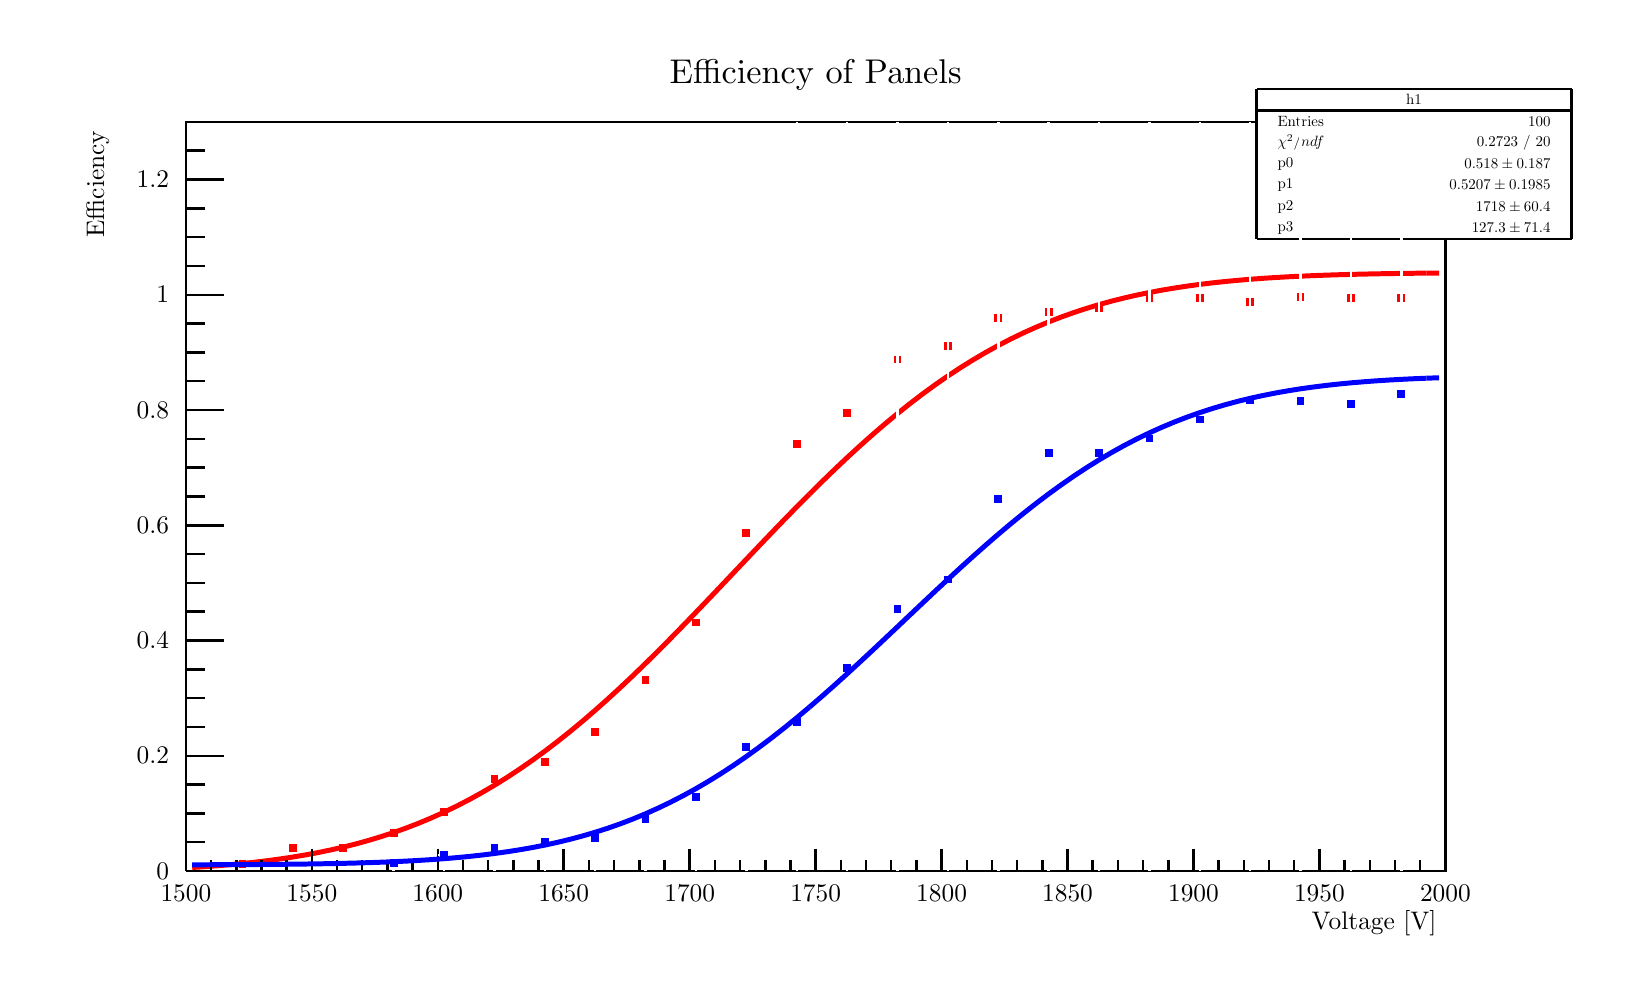
\begin{tikzpicture}
\pgfdeclareplotmark{cross} {
\pgfpathmoveto{\pgfpoint{-0.3\pgfplotmarksize}{\pgfplotmarksize}}
\pgfpathlineto{\pgfpoint{+0.3\pgfplotmarksize}{\pgfplotmarksize}}
\pgfpathlineto{\pgfpoint{+0.3\pgfplotmarksize}{0.3\pgfplotmarksize}}
\pgfpathlineto{\pgfpoint{+1\pgfplotmarksize}{0.3\pgfplotmarksize}}
\pgfpathlineto{\pgfpoint{+1\pgfplotmarksize}{-0.3\pgfplotmarksize}}
\pgfpathlineto{\pgfpoint{+0.3\pgfplotmarksize}{-0.3\pgfplotmarksize}}
\pgfpathlineto{\pgfpoint{+0.3\pgfplotmarksize}{-1.\pgfplotmarksize}}
\pgfpathlineto{\pgfpoint{-0.3\pgfplotmarksize}{-1.\pgfplotmarksize}}
\pgfpathlineto{\pgfpoint{-0.3\pgfplotmarksize}{-0.3\pgfplotmarksize}}
\pgfpathlineto{\pgfpoint{-1.\pgfplotmarksize}{-0.3\pgfplotmarksize}}
\pgfpathlineto{\pgfpoint{-1.\pgfplotmarksize}{0.3\pgfplotmarksize}}
\pgfpathlineto{\pgfpoint{-0.3\pgfplotmarksize}{0.3\pgfplotmarksize}}
\pgfpathclose
\pgfusepathqstroke
}
\pgfdeclareplotmark{cross*} {
\pgfpathmoveto{\pgfpoint{-0.3\pgfplotmarksize}{\pgfplotmarksize}}
\pgfpathlineto{\pgfpoint{+0.3\pgfplotmarksize}{\pgfplotmarksize}}
\pgfpathlineto{\pgfpoint{+0.3\pgfplotmarksize}{0.3\pgfplotmarksize}}
\pgfpathlineto{\pgfpoint{+1\pgfplotmarksize}{0.3\pgfplotmarksize}}
\pgfpathlineto{\pgfpoint{+1\pgfplotmarksize}{-0.3\pgfplotmarksize}}
\pgfpathlineto{\pgfpoint{+0.3\pgfplotmarksize}{-0.3\pgfplotmarksize}}
\pgfpathlineto{\pgfpoint{+0.3\pgfplotmarksize}{-1.\pgfplotmarksize}}
\pgfpathlineto{\pgfpoint{-0.3\pgfplotmarksize}{-1.\pgfplotmarksize}}
\pgfpathlineto{\pgfpoint{-0.3\pgfplotmarksize}{-0.3\pgfplotmarksize}}
\pgfpathlineto{\pgfpoint{-1.\pgfplotmarksize}{-0.3\pgfplotmarksize}}
\pgfpathlineto{\pgfpoint{-1.\pgfplotmarksize}{0.3\pgfplotmarksize}}
\pgfpathlineto{\pgfpoint{-0.3\pgfplotmarksize}{0.3\pgfplotmarksize}}
\pgfpathclose
\pgfusepathqfillstroke
}
\pgfdeclareplotmark{newstar} {
\pgfpathmoveto{\pgfqpoint{0pt}{\pgfplotmarksize}}
\pgfpathlineto{\pgfqpointpolar{44}{0.5\pgfplotmarksize}}
\pgfpathlineto{\pgfqpointpolar{18}{\pgfplotmarksize}}
\pgfpathlineto{\pgfqpointpolar{-20}{0.5\pgfplotmarksize}}
\pgfpathlineto{\pgfqpointpolar{-54}{\pgfplotmarksize}}
\pgfpathlineto{\pgfqpointpolar{-90}{0.5\pgfplotmarksize}}
\pgfpathlineto{\pgfqpointpolar{234}{\pgfplotmarksize}}
\pgfpathlineto{\pgfqpointpolar{198}{0.5\pgfplotmarksize}}
\pgfpathlineto{\pgfqpointpolar{162}{\pgfplotmarksize}}
\pgfpathlineto{\pgfqpointpolar{134}{0.5\pgfplotmarksize}}
\pgfpathclose
\pgfusepathqstroke
}
\pgfdeclareplotmark{newstar*} {
\pgfpathmoveto{\pgfqpoint{0pt}{\pgfplotmarksize}}
\pgfpathlineto{\pgfqpointpolar{44}{0.5\pgfplotmarksize}}
\pgfpathlineto{\pgfqpointpolar{18}{\pgfplotmarksize}}
\pgfpathlineto{\pgfqpointpolar{-20}{0.5\pgfplotmarksize}}
\pgfpathlineto{\pgfqpointpolar{-54}{\pgfplotmarksize}}
\pgfpathlineto{\pgfqpointpolar{-90}{0.5\pgfplotmarksize}}
\pgfpathlineto{\pgfqpointpolar{234}{\pgfplotmarksize}}
\pgfpathlineto{\pgfqpointpolar{198}{0.5\pgfplotmarksize}}
\pgfpathlineto{\pgfqpointpolar{162}{\pgfplotmarksize}}
\pgfpathlineto{\pgfqpointpolar{134}{0.5\pgfplotmarksize}}
\pgfpathclose
\pgfusepathqfillstroke
}
\definecolor{c}{rgb}{1,1,1};
\draw [color=c, fill=c] (0,0) rectangle (20,11.8932);
\draw [color=c, fill=c] (2.00243,1.18932) rectangle (17.9976,10.7039);
\definecolor{c}{rgb}{0,0,0};
\draw [c,line width=0.9] (2.00243,1.18932) -- (2.00243,10.7039) -- (17.9976,10.7039) -- (17.9976,1.18932) -- (2.00243,1.18932);
\definecolor{c}{rgb}{1,1,1};
\draw [color=c, fill=c] (2.00243,1.18932) rectangle (17.9976,10.7039);
\definecolor{c}{rgb}{0,0,0};
\draw [c,line width=0.9] (2.00243,1.18932) -- (2.00243,10.7039) -- (17.9976,10.7039) -- (17.9976,1.18932) -- (2.00243,1.18932);
\definecolor{c}{rgb}{1,1,1};
\draw [c,line width=0.9] (2.72221,1.18932) -- (2.72221,1.22843);
\draw [c,line width=0.9] (2.72221,1.32552) -- (2.72221,1.36462);
\draw [c,line width=0.9] (2.64223,1.27697) -- (2.67367,1.27697);
\draw [c,line width=0.9] (2.77075,1.27697) -- (2.80218,1.27697);
\definecolor{c}{rgb}{1,0,0};
\foreach \P in {(2.72221,1.27697)}{\draw[mark options={color=c,fill=c},mark size=1.201201pt,mark=square*] plot coordinates {\P};}
\definecolor{c}{rgb}{1,1,1};
\draw [c,line width=0.9] (3.36201,1.18932) -- (3.36201,1.43237);
\draw [c,line width=0.9] (3.36201,1.52945) -- (3.36201,1.7725);
\draw [c,line width=0.9] (3.28204,1.48091) -- (3.31347,1.48091);
\draw [c,line width=0.9] (3.41056,1.48091) -- (3.44199,1.48091);
\definecolor{c}{rgb}{1,0,0};
\foreach \P in {(3.36201,1.48091)}{\draw[mark options={color=c,fill=c},mark size=1.201201pt,mark=square*] plot coordinates {\P};}
\definecolor{c}{rgb}{1,1,1};
\draw [c,line width=0.9] (4.00182,1.18932) -- (4.00182,1.43295);
\draw [c,line width=0.9] (4.00182,1.53004) -- (4.00182,1.77366);
\draw [c,line width=0.9] (3.92184,1.48149) -- (3.95328,1.48149);
\draw [c,line width=0.9] (4.05036,1.48149) -- (4.0818,1.48149);
\definecolor{c}{rgb}{1,0,0};
\foreach \P in {(4.00182,1.48149)}{\draw[mark options={color=c,fill=c},mark size=1.201201pt,mark=square*] plot coordinates {\P};}
\definecolor{c}{rgb}{1,1,1};
\draw [c,line width=0.9] (4.64163,1.18932) -- (4.64163,1.62382);
\draw [c,line width=0.9] (4.64163,1.72091) -- (4.64163,2.15541);
\draw [c,line width=0.9] (4.56165,1.67237) -- (4.59308,1.67237);
\draw [c,line width=0.9] (4.69017,1.67237) -- (4.7216,1.67237);
\definecolor{c}{rgb}{1,0,0};
\foreach \P in {(4.64163,1.67237)}{\draw[mark options={color=c,fill=c},mark size=1.201201pt,mark=square*] plot coordinates {\P};}
\definecolor{c}{rgb}{1,1,1};
\draw [c,line width=0.9] (5.28143,1.18932) -- (5.28143,1.89181);
\draw [c,line width=0.9] (5.28143,1.9889) -- (5.28143,2.69139);
\draw [c,line width=0.9] (5.20146,1.94036) -- (5.23289,1.94036);
\draw [c,line width=0.9] (5.32998,1.94036) -- (5.36141,1.94036);
\definecolor{c}{rgb}{1,0,0};
\foreach \P in {(5.28143,1.94036)}{\draw[mark options={color=c,fill=c},mark size=1.201201pt,mark=square*] plot coordinates {\P};}
\definecolor{c}{rgb}{1,1,1};
\draw [c,line width=0.9] (5.92124,1.18932) -- (5.92124,2.30714);
\draw [c,line width=0.9] (5.92124,2.40423) -- (5.92124,3.52204);
\draw [c,line width=0.9] (5.84126,2.35568) -- (5.87269,2.35568);
\draw [c,line width=0.9] (5.96978,2.35568) -- (6.00121,2.35568);
\definecolor{c}{rgb}{1,0,0};
\foreach \P in {(5.92124,2.35568)}{\draw[mark options={color=c,fill=c},mark size=1.201201pt,mark=square*] plot coordinates {\P};}
\definecolor{c}{rgb}{1,1,1};
\draw [c,line width=0.9] (6.56104,1.18932) -- (6.56104,2.52307);
\draw [c,line width=0.9] (6.56104,2.62016) -- (6.56104,3.95392);
\draw [c,line width=0.9] (6.48107,2.57162) -- (6.5125,2.57162);
\draw [c,line width=0.9] (6.60959,2.57162) -- (6.64102,2.57162);
\definecolor{c}{rgb}{1,0,0};
\foreach \P in {(6.56104,2.57162)}{\draw[mark options={color=c,fill=c},mark size=1.201201pt,mark=square*] plot coordinates {\P};}
\definecolor{c}{rgb}{1,1,1};
\draw [c,line width=0.9] (7.20085,1.18932) -- (7.20085,2.90841);
\draw [c,line width=0.9] (7.20085,3.0055) -- (7.20085,4.7246);
\draw [c,line width=0.9] (7.12087,2.95696) -- (7.15231,2.95696);
\draw [c,line width=0.9] (7.24939,2.95696) -- (7.28083,2.95696);
\definecolor{c}{rgb}{1,0,0};
\foreach \P in {(7.20085,2.95696)}{\draw[mark options={color=c,fill=c},mark size=1.201201pt,mark=square*] plot coordinates {\P};}
\definecolor{c}{rgb}{1,1,1};
\draw [c,line width=0.9] (7.84066,1.18932) -- (7.84066,3.5658);
\draw [c,line width=0.9] (7.84066,3.66288) -- (7.84066,6.03936);
\draw [c,line width=0.9] (7.76068,3.61434) -- (7.79211,3.61434);
\draw [c,line width=0.9] (7.8892,3.61434) -- (7.92063,3.61434);
\definecolor{c}{rgb}{1,0,0};
\foreach \P in {(7.84066,3.61434)}{\draw[mark options={color=c,fill=c},mark size=1.201201pt,mark=square*] plot coordinates {\P};}
\definecolor{c}{rgb}{1,1,1};
\draw [c,line width=0.9] (8.48046,1.18932) -- (8.48046,4.29853);
\draw [c,line width=0.9] (8.48046,4.39562) -- (8.48046,7.50482);
\draw [c,line width=0.9] (8.40049,4.34707) -- (8.43192,4.34707);
\draw [c,line width=0.9] (8.52901,4.34707) -- (8.56044,4.34707);
\definecolor{c}{rgb}{1,0,0};
\foreach \P in {(8.48046,4.34707)}{\draw[mark options={color=c,fill=c},mark size=1.201201pt,mark=square*] plot coordinates {\P};}
\definecolor{c}{rgb}{1,1,1};
\draw [c,line width=0.9] (9.12027,1.18932) -- (9.12027,5.43824);
\draw [c,line width=0.9] (9.12027,5.53533) -- (9.12027,9.78425);
\draw [c,line width=0.9] (9.04029,5.48678) -- (9.07172,5.48678);
\draw [c,line width=0.9] (9.16881,5.48678) -- (9.20024,5.48678);
\definecolor{c}{rgb}{1,0,0};
\foreach \P in {(9.12027,5.48678)}{\draw[mark options={color=c,fill=c},mark size=1.201201pt,mark=square*] plot coordinates {\P};}
\definecolor{c}{rgb}{1,1,1};
\draw [c,line width=0.9] (9.76007,1.18932) -- (9.76007,6.56486);
\draw [c,line width=0.9] (9.76007,6.66195) -- (9.76007,10.7039);
\draw [c,line width=0.9] (9.6801,6.6134) -- (9.71153,6.6134);
\draw [c,line width=0.9] (9.80862,6.6134) -- (9.84005,6.6134);
\definecolor{c}{rgb}{1,0,0};
\foreach \P in {(9.76007,6.6134)}{\draw[mark options={color=c,fill=c},mark size=1.201201pt,mark=square*] plot coordinates {\P};}
\definecolor{c}{rgb}{1,1,1};
\draw [c,line width=0.9] (10.3999,1.18932) -- (10.3999,6.96062);
\draw [c,line width=0.9] (10.3999,7.05771) -- (10.3999,10.7039);
\draw [c,line width=0.9] (10.3199,7.00917) -- (10.3513,7.00917);
\draw [c,line width=0.9] (10.4484,7.00917) -- (10.4799,7.00917);
\definecolor{c}{rgb}{1,0,0};
\foreach \P in {(10.3999,7.00917)}{\draw[mark options={color=c,fill=c},mark size=1.201201pt,mark=square*] plot coordinates {\P};}
\definecolor{c}{rgb}{1,1,1};
\draw [c,line width=0.9] (11.0397,1.18932) -- (11.0397,7.63666);
\draw [c,line width=0.9] (11.0397,7.73375) -- (11.0397,10.7039);
\draw [c,line width=0.9] (10.9597,7.6852) -- (10.9911,7.6852);
\draw [c,line width=0.9] (11.0882,7.6852) -- (11.1197,7.6852);
\definecolor{c}{rgb}{1,0,0};
\foreach \P in {(11.0397,7.6852)}{\draw[mark options={color=c,fill=c},mark size=1.201201pt,mark=square*] plot coordinates {\P};}
\definecolor{c}{rgb}{1,1,1};
\draw [c,line width=0.9] (11.6795,1.18932) -- (11.6795,7.81302);
\draw [c,line width=0.9] (11.6795,7.91011) -- (11.6795,10.7039);
\draw [c,line width=0.9] (11.5995,7.86157) -- (11.6309,7.86157);
\draw [c,line width=0.9] (11.728,7.86157) -- (11.7595,7.86157);
\definecolor{c}{rgb}{1,0,0};
\foreach \P in {(11.6795,7.86157)}{\draw[mark options={color=c,fill=c},mark size=1.201201pt,mark=square*] plot coordinates {\P};}
\definecolor{c}{rgb}{1,1,1};
\draw [c,line width=0.9] (12.3193,1.18932) -- (12.3193,8.16924);
\draw [c,line width=0.9] (12.3193,8.26632) -- (12.3193,10.7039);
\draw [c,line width=0.9] (12.2393,8.21778) -- (12.2708,8.21778);
\draw [c,line width=0.9] (12.3678,8.21778) -- (12.3993,8.21778);
\definecolor{c}{rgb}{1,0,0};
\foreach \P in {(12.3193,8.21778)}{\draw[mark options={color=c,fill=c},mark size=1.201201pt,mark=square*] plot coordinates {\P};}
\definecolor{c}{rgb}{1,1,1};
\draw [c,line width=0.9] (12.9591,1.18932) -- (12.9591,8.23923);
\draw [c,line width=0.9] (12.9591,8.33631) -- (12.9591,10.7039);
\draw [c,line width=0.9] (12.8791,8.28777) -- (12.9106,8.28777);
\draw [c,line width=0.9] (13.0076,8.28777) -- (13.0391,8.28777);
\definecolor{c}{rgb}{1,0,0};
\foreach \P in {(12.9591,8.28777)}{\draw[mark options={color=c,fill=c},mark size=1.201201pt,mark=square*] plot coordinates {\P};}
\definecolor{c}{rgb}{1,1,1};
\draw [c,line width=0.9] (13.5989,1.18932) -- (13.5989,8.28506);
\draw [c,line width=0.9] (13.5989,8.38215) -- (13.5989,10.7039);
\draw [c,line width=0.9] (13.5189,8.33361) -- (13.5504,8.33361);
\draw [c,line width=0.9] (13.6475,8.33361) -- (13.6789,8.33361);
\definecolor{c}{rgb}{1,0,0};
\foreach \P in {(13.5989,8.33361)}{\draw[mark options={color=c,fill=c},mark size=1.201201pt,mark=square*] plot coordinates {\P};}
\definecolor{c}{rgb}{1,1,1};
\draw [c,line width=0.9] (14.2387,1.18932) -- (14.2387,8.41567);
\draw [c,line width=0.9] (14.2387,8.51276) -- (14.2387,10.7039);
\draw [c,line width=0.9] (14.1587,8.46421) -- (14.1902,8.46421);
\draw [c,line width=0.9] (14.2873,8.46421) -- (14.3187,8.46421);
\definecolor{c}{rgb}{1,0,0};
\foreach \P in {(14.2387,8.46421)}{\draw[mark options={color=c,fill=c},mark size=1.201201pt,mark=square*] plot coordinates {\P};}
\definecolor{c}{rgb}{1,1,1};
\draw [c,line width=0.9] (14.8785,1.18932) -- (14.8785,8.41585);
\draw [c,line width=0.9] (14.8785,8.51293) -- (14.8785,10.7039);
\draw [c,line width=0.9] (14.7985,8.46439) -- (14.83,8.46439);
\draw [c,line width=0.9] (14.9271,8.46439) -- (14.9585,8.46439);
\definecolor{c}{rgb}{1,0,0};
\foreach \P in {(14.8785,8.46439)}{\draw[mark options={color=c,fill=c},mark size=1.201201pt,mark=square*] plot coordinates {\P};}
\definecolor{c}{rgb}{1,1,1};
\draw [c,line width=0.9] (15.5183,1.18932) -- (15.5183,8.37237);
\draw [c,line width=0.9] (15.5183,8.46946) -- (15.5183,10.7039);
\draw [c,line width=0.9] (15.4383,8.42091) -- (15.4698,8.42091);
\draw [c,line width=0.9] (15.5669,8.42091) -- (15.5983,8.42091);
\definecolor{c}{rgb}{1,0,0};
\foreach \P in {(15.5183,8.42091)}{\draw[mark options={color=c,fill=c},mark size=1.201201pt,mark=square*] plot coordinates {\P};}
\definecolor{c}{rgb}{1,1,1};
\draw [c,line width=0.9] (16.1581,1.18932) -- (16.1581,8.43063);
\draw [c,line width=0.9] (16.1581,8.52772) -- (16.1581,10.7039);
\draw [c,line width=0.9] (16.0782,8.47917) -- (16.1096,8.47917);
\draw [c,line width=0.9] (16.2067,8.47917) -- (16.2381,8.47917);
\definecolor{c}{rgb}{1,0,0};
\foreach \P in {(16.1581,8.47917)}{\draw[mark options={color=c,fill=c},mark size=1.201201pt,mark=square*] plot coordinates {\P};}
\definecolor{c}{rgb}{1,1,1};
\draw [c,line width=0.9] (16.7979,1.18932) -- (16.7979,8.41541);
\draw [c,line width=0.9] (16.7979,8.51249) -- (16.7979,10.7039);
\draw [c,line width=0.9] (16.718,8.46395) -- (16.7494,8.46395);
\draw [c,line width=0.9] (16.8465,8.46395) -- (16.8779,8.46395);
\definecolor{c}{rgb}{1,0,0};
\foreach \P in {(16.7979,8.46395)}{\draw[mark options={color=c,fill=c},mark size=1.201201pt,mark=square*] plot coordinates {\P};}
\definecolor{c}{rgb}{1,1,1};
\draw [c,line width=0.9] (17.4377,1.18932) -- (17.4377,8.41585);
\draw [c,line width=0.9] (17.4377,8.51293) -- (17.4377,10.7039);
\draw [c,line width=0.9] (17.3578,8.46439) -- (17.3892,8.46439);
\draw [c,line width=0.9] (17.4863,8.46439) -- (17.5177,8.46439);
\definecolor{c}{rgb}{1,0,0};
\foreach \P in {(17.4377,8.46439)}{\draw[mark options={color=c,fill=c},mark size=1.201201pt,mark=square*] plot coordinates {\P};}
\draw [c,line width=1.8] (2.0824,1.2344) -- (2.24235,1.2448) -- (2.40231,1.25664) -- (2.56226,1.27008) -- (2.72221,1.28528) -- (2.88216,1.30243) -- (3.04211,1.32171) -- (3.20206,1.34332) -- (3.36201,1.36748) -- (3.52197,1.39439) -- (3.68192,1.42427)
 -- (3.84187,1.45736) -- (4.00182,1.49389) -- (4.16177,1.53408) -- (4.32172,1.57817) -- (4.48167,1.62639) -- (4.64163,1.67896) -- (4.80158,1.7361) -- (4.96153,1.79802) -- (5.12148,1.8649) -- (5.28143,1.93692) -- (5.44138,2.01425) -- (5.60134,2.097)
 -- (5.76129,2.1853) -- (5.92124,2.27922) -- (6.08119,2.37881) -- (6.24114,2.48409) -- (6.40109,2.59504) -- (6.56104,2.71161) -- (6.721,2.8337) -- (6.88095,2.96119) -- (7.0409,3.09389) -- (7.20085,3.2316) -- (7.3608,3.37407) -- (7.52075,3.52101) --
 (7.6807,3.67208) -- (7.84066,3.82694) -- (8.00061,3.98517) -- (8.16056,4.14637) -- (8.32051,4.31007) -- (8.48046,4.47581) -- (8.64041,4.64309) -- (8.80036,4.8114) -- (8.96032,4.98024) -- (9.12027,5.14908) -- (9.28022,5.31741) -- (9.44017,5.4847) --
 (9.60012,5.65044) -- (9.76007,5.81416) -- (9.92002,5.97537);
\draw [c,line width=1.8] (9.92002,5.97537) -- (10.08,6.13363) -- (10.2399,6.2885) -- (10.3999,6.4396) -- (10.5598,6.58656) -- (10.7198,6.72906) -- (10.8797,6.8668) -- (11.0397,6.99954) -- (11.1996,7.12706) -- (11.3596,7.24918) -- (11.5195,7.36579) --
 (11.6795,7.47678) -- (11.8394,7.58209) -- (11.9994,7.68172) -- (12.1593,7.77567) -- (12.3193,7.864) -- (12.4792,7.94679) -- (12.6392,8.02415) -- (12.7992,8.0962) -- (12.9591,8.16311) -- (13.1191,8.22506) -- (13.279,8.28223) -- (13.439,8.33483) --
 (13.5989,8.38307) -- (13.7589,8.42719) -- (13.9188,8.4674) -- (14.0788,8.50395) -- (14.2387,8.53706) -- (14.3987,8.56697) -- (14.5586,8.59389) -- (14.7186,8.61806) -- (14.8785,8.63969) -- (15.0385,8.65899) -- (15.1984,8.67615) -- (15.3584,8.69136)
 -- (15.5183,8.70481) -- (15.6783,8.71666) -- (15.8382,8.72707) -- (15.9982,8.73619) -- (16.1581,8.74414) -- (16.3181,8.75107) -- (16.478,8.75708) -- (16.638,8.76228) -- (16.7979,8.76676) -- (16.9579,8.77062) -- (17.1178,8.77392) -- (17.2778,8.77674)
 -- (17.4377,8.77914) -- (17.5977,8.78119) -- (17.7576,8.78291);
\draw [c,line width=1.8] (17.7576,8.78291) -- (17.9176,8.78437);
\definecolor{c}{rgb}{1,1,1};
\draw [color=c, fill=c] (15.6,9.21723) rectangle (19.6,11.1201);
\definecolor{c}{rgb}{0,0,0};
\draw [c,line width=0.9] (15.6,9.21723) -- (19.6,9.21723);
\draw [c,line width=0.9] (19.6,9.21723) -- (19.6,11.1201);
\draw [c,line width=0.9] (19.6,11.1201) -- (15.6,11.1201);
\draw [c,line width=0.9] (15.6,11.1201) -- (15.6,9.21723);
\draw (17.6,10.9842) node[scale=0.53907, color=c, rotate=0]{h1};
\draw [c,line width=0.9] (15.6,10.8483) -- (19.6,10.8483);
\draw [anchor= west] (15.8,10.7124) node[scale=0.53907, color=c, rotate=0]{Entries };
\draw [anchor= east] (19.4,10.7124) node[scale=0.53907, color=c, rotate=0]{ 100};
\draw [anchor= west] (15.8,10.4405) node[scale=0.53907, color=c, rotate=0]{$\chi^{2} / ndf $};
\draw [anchor= east] (19.4,10.4405) node[scale=0.53907, color=c, rotate=0]{ 0.2723 / 20};
\draw [anchor= west] (15.8,10.1687) node[scale=0.53907, color=c, rotate=0]{p0       };
\draw [anchor= east] (19.4,10.1687) node[scale=0.53907, color=c, rotate=0]{$ 0.518 \pm 0.187$};
\draw [anchor= west] (15.8,9.89684) node[scale=0.53907, color=c, rotate=0]{p1       };
\draw [anchor= east] (19.4,9.89684) node[scale=0.53907, color=c, rotate=0]{$ 0.5207 \pm 0.1985$};
\draw [anchor= west] (15.8,9.625) node[scale=0.53907, color=c, rotate=0]{p2       };
\draw [anchor= east] (19.4,9.625) node[scale=0.53907, color=c, rotate=0]{$  1718 \pm 60.4$};
\draw [anchor= west] (15.8,9.35316) node[scale=0.53907, color=c, rotate=0]{p3       };
\draw [anchor= east] (19.4,9.35316) node[scale=0.53907, color=c, rotate=0]{$ 127.3 \pm 71.4$};
\draw [c,line width=0.9] (2.00243,1.18932) -- (17.9976,1.18932);
\draw [anchor= east] (17.9976,0.523301) node[scale=0.91642, color=c, rotate=0]{Voltage [V]};
\draw [c,line width=0.9] (2.00243,1.47467) -- (2.00243,1.18932);
\draw [c,line width=0.9] (2.32233,1.332) -- (2.32233,1.18932);
\draw [c,line width=0.9] (2.64223,1.332) -- (2.64223,1.18932);
\draw [c,line width=0.9] (2.96214,1.332) -- (2.96214,1.18932);
\draw [c,line width=0.9] (3.28204,1.332) -- (3.28204,1.18932);
\draw [c,line width=0.9] (3.60194,1.47467) -- (3.60194,1.18932);
\draw [c,line width=0.9] (3.92184,1.332) -- (3.92184,1.18932);
\draw [c,line width=0.9] (4.24175,1.332) -- (4.24175,1.18932);
\draw [c,line width=0.9] (4.56165,1.332) -- (4.56165,1.18932);
\draw [c,line width=0.9] (4.88155,1.332) -- (4.88155,1.18932);
\draw [c,line width=0.9] (5.20146,1.47467) -- (5.20146,1.18932);
\draw [c,line width=0.9] (5.52136,1.332) -- (5.52136,1.18932);
\draw [c,line width=0.9] (5.84126,1.332) -- (5.84126,1.18932);
\draw [c,line width=0.9] (6.16117,1.332) -- (6.16117,1.18932);
\draw [c,line width=0.9] (6.48107,1.332) -- (6.48107,1.18932);
\draw [c,line width=0.9] (6.80097,1.47467) -- (6.80097,1.18932);
\draw [c,line width=0.9] (7.12087,1.332) -- (7.12087,1.18932);
\draw [c,line width=0.9] (7.44078,1.332) -- (7.44078,1.18932);
\draw [c,line width=0.9] (7.76068,1.332) -- (7.76068,1.18932);
\draw [c,line width=0.9] (8.08058,1.332) -- (8.08058,1.18932);
\draw [c,line width=0.9] (8.40049,1.47467) -- (8.40049,1.18932);
\draw [c,line width=0.9] (8.72039,1.332) -- (8.72039,1.18932);
\draw [c,line width=0.9] (9.04029,1.332) -- (9.04029,1.18932);
\draw [c,line width=0.9] (9.36019,1.332) -- (9.36019,1.18932);
\draw [c,line width=0.9] (9.6801,1.332) -- (9.6801,1.18932);
\draw [c,line width=0.9] (10,1.47467) -- (10,1.18932);
\draw [c,line width=0.9] (10.3199,1.332) -- (10.3199,1.18932);
\draw [c,line width=0.9] (10.6398,1.332) -- (10.6398,1.18932);
\draw [c,line width=0.9] (10.9597,1.332) -- (10.9597,1.18932);
\draw [c,line width=0.9] (11.2796,1.332) -- (11.2796,1.18932);
\draw [c,line width=0.9] (11.5995,1.47467) -- (11.5995,1.18932);
\draw [c,line width=0.9] (11.9194,1.332) -- (11.9194,1.18932);
\draw [c,line width=0.9] (12.2393,1.332) -- (12.2393,1.18932);
\draw [c,line width=0.9] (12.5592,1.332) -- (12.5592,1.18932);
\draw [c,line width=0.9] (12.8791,1.332) -- (12.8791,1.18932);
\draw [c,line width=0.9] (13.199,1.47467) -- (13.199,1.18932);
\draw [c,line width=0.9] (13.5189,1.332) -- (13.5189,1.18932);
\draw [c,line width=0.9] (13.8388,1.332) -- (13.8388,1.18932);
\draw [c,line width=0.9] (14.1587,1.332) -- (14.1587,1.18932);
\draw [c,line width=0.9] (14.4786,1.332) -- (14.4786,1.18932);
\draw [c,line width=0.9] (14.7985,1.47467) -- (14.7985,1.18932);
\draw [c,line width=0.9] (15.1184,1.332) -- (15.1184,1.18932);
\draw [c,line width=0.9] (15.4383,1.332) -- (15.4383,1.18932);
\draw [c,line width=0.9] (15.7583,1.332) -- (15.7583,1.18932);
\draw [c,line width=0.9] (16.0782,1.332) -- (16.0782,1.18932);
\draw [c,line width=0.9] (16.3981,1.47467) -- (16.3981,1.18932);
\draw [c,line width=0.9] (16.718,1.332) -- (16.718,1.18932);
\draw [c,line width=0.9] (17.0379,1.332) -- (17.0379,1.18932);
\draw [c,line width=0.9] (17.3578,1.332) -- (17.3578,1.18932);
\draw [c,line width=0.9] (17.6777,1.332) -- (17.6777,1.18932);
\draw [c,line width=0.9] (17.9976,1.47467) -- (17.9976,1.18932);
\draw [anchor=base] (2.00243,0.796845) node[scale=0.91642, color=c, rotate=0]{1500};
\draw [anchor=base] (3.60194,0.796845) node[scale=0.91642, color=c, rotate=0]{1550};
\draw [anchor=base] (5.20146,0.796845) node[scale=0.91642, color=c, rotate=0]{1600};
\draw [anchor=base] (6.80097,0.796845) node[scale=0.91642, color=c, rotate=0]{1650};
\draw [anchor=base] (8.40049,0.796845) node[scale=0.91642, color=c, rotate=0]{1700};
\draw [anchor=base] (10,0.796845) node[scale=0.91642, color=c, rotate=0]{1750};
\draw [anchor=base] (11.5995,0.796845) node[scale=0.91642, color=c, rotate=0]{1800};
\draw [anchor=base] (13.199,0.796845) node[scale=0.91642, color=c, rotate=0]{1850};
\draw [anchor=base] (14.7985,0.796845) node[scale=0.91642, color=c, rotate=0]{1900};
\draw [anchor=base] (16.3981,0.796845) node[scale=0.91642, color=c, rotate=0]{1950};
\draw [anchor=base] (17.9976,0.796845) node[scale=0.91642, color=c, rotate=0]{2000};
\draw [c,line width=0.9] (2.00243,1.18932) -- (2.00243,10.7039);
\draw [anchor= east] (0.882427,10.7039) node[scale=0.91642, color=c, rotate=90]{Efficiency};
\draw [c,line width=0.9] (2.48243,1.18932) -- (2.00243,1.18932);
\draw [c,line width=0.9] (2.24243,1.55527) -- (2.00243,1.55527);
\draw [c,line width=0.9] (2.24243,1.92121) -- (2.00243,1.92121);
\draw [c,line width=0.9] (2.24243,2.28715) -- (2.00243,2.28715);
\draw [c,line width=0.9] (2.48243,2.6531) -- (2.00243,2.6531);
\draw [c,line width=0.9] (2.24243,3.01904) -- (2.00243,3.01904);
\draw [c,line width=0.9] (2.24243,3.38499) -- (2.00243,3.38499);
\draw [c,line width=0.9] (2.24243,3.75093) -- (2.00243,3.75093);
\draw [c,line width=0.9] (2.48243,4.11688) -- (2.00243,4.11688);
\draw [c,line width=0.9] (2.24243,4.48282) -- (2.00243,4.48282);
\draw [c,line width=0.9] (2.24243,4.84877) -- (2.00243,4.84877);
\draw [c,line width=0.9] (2.24243,5.21471) -- (2.00243,5.21471);
\draw [c,line width=0.9] (2.48243,5.58066) -- (2.00243,5.58066);
\draw [c,line width=0.9] (2.24243,5.9466) -- (2.00243,5.9466);
\draw [c,line width=0.9] (2.24243,6.31255) -- (2.00243,6.31255);
\draw [c,line width=0.9] (2.24243,6.67849) -- (2.00243,6.67849);
\draw [c,line width=0.9] (2.48243,7.04444) -- (2.00243,7.04444);
\draw [c,line width=0.9] (2.24243,7.41038) -- (2.00243,7.41038);
\draw [c,line width=0.9] (2.24243,7.77633) -- (2.00243,7.77633);
\draw [c,line width=0.9] (2.24243,8.14227) -- (2.00243,8.14227);
\draw [c,line width=0.9] (2.48243,8.50821) -- (2.00243,8.50821);
\draw [c,line width=0.9] (2.24243,8.87416) -- (2.00243,8.87416);
\draw [c,line width=0.9] (2.24243,9.2401) -- (2.00243,9.2401);
\draw [c,line width=0.9] (2.24243,9.60605) -- (2.00243,9.60605);
\draw [c,line width=0.9] (2.48243,9.97199) -- (2.00243,9.97199);
\draw [c,line width=0.9] (2.48243,9.97199) -- (2.00243,9.97199);
\draw [c,line width=0.9] (2.24243,10.3379) -- (2.00243,10.3379);
\draw [anchor= east] (1.90243,1.18932) node[scale=0.91642, color=c, rotate=0]{0};
\draw [anchor= east] (1.90243,2.6531) node[scale=0.91642, color=c, rotate=0]{0.2};
\draw [anchor= east] (1.90243,4.11688) node[scale=0.91642, color=c, rotate=0]{0.4};
\draw [anchor= east] (1.90243,5.58066) node[scale=0.91642, color=c, rotate=0]{0.6};
\draw [anchor= east] (1.90243,7.04444) node[scale=0.91642, color=c, rotate=0]{0.8};
\draw [anchor= east] (1.90243,8.50821) node[scale=0.91642, color=c, rotate=0]{1};
\draw [anchor= east] (1.90243,9.97199) node[scale=0.91642, color=c, rotate=0]{1.2};
\definecolor{c}{rgb}{1,1,1};
\draw [color=c, fill=c] (15.6,9.21723) rectangle (19.6,11.1201);
\definecolor{c}{rgb}{0,0,0};
\draw [c,line width=0.9] (15.6,9.21723) -- (19.6,9.21723);
\draw [c,line width=0.9] (19.6,9.21723) -- (19.6,11.1201);
\draw [c,line width=0.9] (19.6,11.1201) -- (15.6,11.1201);
\draw [c,line width=0.9] (15.6,11.1201) -- (15.6,9.21723);
\draw (17.6,10.9842) node[scale=0.53907, color=c, rotate=0]{h1};
\draw [c,line width=0.9] (15.6,10.8483) -- (19.6,10.8483);
\draw [anchor= west] (15.8,10.7124) node[scale=0.53907, color=c, rotate=0]{Entries };
\draw [anchor= east] (19.4,10.7124) node[scale=0.53907, color=c, rotate=0]{ 100};
\draw [anchor= west] (15.8,10.4405) node[scale=0.53907, color=c, rotate=0]{$\chi^{2} / ndf $};
\draw [anchor= east] (19.4,10.4405) node[scale=0.53907, color=c, rotate=0]{ 0.2723 / 20};
\draw [anchor= west] (15.8,10.1687) node[scale=0.53907, color=c, rotate=0]{p0       };
\draw [anchor= east] (19.4,10.1687) node[scale=0.53907, color=c, rotate=0]{$ 0.518 \pm 0.187$};
\draw [anchor= west] (15.8,9.89684) node[scale=0.53907, color=c, rotate=0]{p1       };
\draw [anchor= east] (19.4,9.89684) node[scale=0.53907, color=c, rotate=0]{$ 0.5207 \pm 0.1985$};
\draw [anchor= west] (15.8,9.625) node[scale=0.53907, color=c, rotate=0]{p2       };
\draw [anchor= east] (19.4,9.625) node[scale=0.53907, color=c, rotate=0]{$  1718 \pm 60.4$};
\draw [anchor= west] (15.8,9.35316) node[scale=0.53907, color=c, rotate=0]{p3       };
\draw [anchor= east] (19.4,9.35316) node[scale=0.53907, color=c, rotate=0]{$ 127.3 \pm 71.4$};
\definecolor{c}{rgb}{1,1,1};
\draw [c,line width=0.9] (4.64163,1.18932) -- (4.64163,1.24283);
\draw [c,line width=0.9] (4.64163,1.33992) -- (4.64163,1.39343);
\draw [c,line width=0.9] (4.56165,1.29138) -- (4.59308,1.29138);
\draw [c,line width=0.9] (4.69017,1.29138) -- (4.7216,1.29138);
\definecolor{c}{rgb}{0,0,1};
\foreach \P in {(4.64163,1.29138)}{\draw[mark options={color=c,fill=c},mark size=1.201201pt,mark=square*] plot coordinates {\P};}
\definecolor{c}{rgb}{1,1,1};
\draw [c,line width=0.9] (5.28143,1.18932) -- (5.28143,1.34448);
\draw [c,line width=0.9] (5.28143,1.44157) -- (5.28143,1.59673);
\draw [c,line width=0.9] (5.20146,1.39303) -- (5.23289,1.39303);
\draw [c,line width=0.9] (5.32998,1.39303) -- (5.36141,1.39303);
\definecolor{c}{rgb}{0,0,1};
\foreach \P in {(5.28143,1.39303)}{\draw[mark options={color=c,fill=c},mark size=1.201201pt,mark=square*] plot coordinates {\P};}
\definecolor{c}{rgb}{1,1,1};
\draw [c,line width=0.9] (5.92124,1.18932) -- (5.92124,1.43179);
\draw [c,line width=0.9] (5.92124,1.52887) -- (5.92124,1.77134);
\draw [c,line width=0.9] (5.84126,1.48033) -- (5.87269,1.48033);
\draw [c,line width=0.9] (5.96978,1.48033) -- (6.00121,1.48033);
\definecolor{c}{rgb}{0,0,1};
\foreach \P in {(5.92124,1.48033)}{\draw[mark options={color=c,fill=c},mark size=1.201201pt,mark=square*] plot coordinates {\P};}
\definecolor{c}{rgb}{1,1,1};
\draw [c,line width=0.9] (6.56104,1.18932) -- (6.56104,1.50672);
\draw [c,line width=0.9] (6.56104,1.60381) -- (6.56104,1.92121);
\draw [c,line width=0.9] (6.48107,1.55527) -- (6.5125,1.55527);
\draw [c,line width=0.9] (6.60959,1.55527) -- (6.64102,1.55527);
\definecolor{c}{rgb}{0,0,1};
\foreach \P in {(6.56104,1.55527)}{\draw[mark options={color=c,fill=c},mark size=1.201201pt,mark=square*] plot coordinates {\P};}
\definecolor{c}{rgb}{1,1,1};
\draw [c,line width=0.9] (7.20085,1.18932) -- (7.20085,1.5619);
\draw [c,line width=0.9] (7.20085,1.65899) -- (7.20085,2.03157);
\draw [c,line width=0.9] (7.12087,1.61045) -- (7.15231,1.61045);
\draw [c,line width=0.9] (7.24939,1.61045) -- (7.28083,1.61045);
\definecolor{c}{rgb}{0,0,1};
\foreach \P in {(7.20085,1.61045)}{\draw[mark options={color=c,fill=c},mark size=1.201201pt,mark=square*] plot coordinates {\P};}
\definecolor{c}{rgb}{1,1,1};
\draw [c,line width=0.9] (7.84066,1.18932) -- (7.84066,1.79816);
\draw [c,line width=0.9] (7.84066,1.89525) -- (7.84066,2.50409);
\draw [c,line width=0.9] (7.76068,1.84671) -- (7.79211,1.84671);
\draw [c,line width=0.9] (7.8892,1.84671) -- (7.92063,1.84671);
\definecolor{c}{rgb}{0,0,1};
\foreach \P in {(7.84066,1.84671)}{\draw[mark options={color=c,fill=c},mark size=1.201201pt,mark=square*] plot coordinates {\P};}
\definecolor{c}{rgb}{1,1,1};
\draw [c,line width=0.9] (8.48046,1.18932) -- (8.48046,2.08468);
\draw [c,line width=0.9] (8.48046,2.18177) -- (8.48046,3.07713);
\draw [c,line width=0.9] (8.40049,2.13322) -- (8.43192,2.13322);
\draw [c,line width=0.9] (8.52901,2.13322) -- (8.56044,2.13322);
\definecolor{c}{rgb}{0,0,1};
\foreach \P in {(8.48046,2.13322)}{\draw[mark options={color=c,fill=c},mark size=1.201201pt,mark=square*] plot coordinates {\P};}
\definecolor{c}{rgb}{1,1,1};
\draw [c,line width=0.9] (9.12027,1.18932) -- (9.12027,2.7185);
\draw [c,line width=0.9] (9.12027,2.81559) -- (9.12027,4.34477);
\draw [c,line width=0.9] (9.04029,2.76705) -- (9.07172,2.76705);
\draw [c,line width=0.9] (9.16881,2.76705) -- (9.20024,2.76705);
\definecolor{c}{rgb}{0,0,1};
\foreach \P in {(9.12027,2.76705)}{\draw[mark options={color=c,fill=c},mark size=1.201201pt,mark=square*] plot coordinates {\P};}
\definecolor{c}{rgb}{1,1,1};
\draw [c,line width=0.9] (9.76007,1.18932) -- (9.76007,3.03234);
\draw [c,line width=0.9] (9.76007,3.12943) -- (9.76007,4.97244);
\draw [c,line width=0.9] (9.6801,3.08088) -- (9.71153,3.08088);
\draw [c,line width=0.9] (9.80862,3.08088) -- (9.84005,3.08088);
\definecolor{c}{rgb}{0,0,1};
\foreach \P in {(9.76007,3.08088)}{\draw[mark options={color=c,fill=c},mark size=1.201201pt,mark=square*] plot coordinates {\P};}
\definecolor{c}{rgb}{1,1,1};
\draw [c,line width=0.9] (10.3999,1.18932) -- (10.3999,3.72219);
\draw [c,line width=0.9] (10.3999,3.81927) -- (10.3999,6.35214);
\draw [c,line width=0.9] (10.3199,3.77073) -- (10.3513,3.77073);
\draw [c,line width=0.9] (10.4484,3.77073) -- (10.4799,3.77073);
\definecolor{c}{rgb}{0,0,1};
\foreach \P in {(10.3999,3.77073)}{\draw[mark options={color=c,fill=c},mark size=1.201201pt,mark=square*] plot coordinates {\P};}
\definecolor{c}{rgb}{1,1,1};
\draw [c,line width=0.9] (11.0397,1.18932) -- (11.0397,4.46489);
\draw [c,line width=0.9] (11.0397,4.56198) -- (11.0397,7.83756);
\draw [c,line width=0.9] (10.9597,4.51344) -- (10.9911,4.51344);
\draw [c,line width=0.9] (11.0882,4.51344) -- (11.1197,4.51344);
\definecolor{c}{rgb}{0,0,1};
\foreach \P in {(11.0397,4.51344)}{\draw[mark options={color=c,fill=c},mark size=1.201201pt,mark=square*] plot coordinates {\P};}
\definecolor{c}{rgb}{1,1,1};
\draw [c,line width=0.9] (11.6795,1.18932) -- (11.6795,4.84414);
\draw [c,line width=0.9] (11.6795,4.94122) -- (11.6795,8.59604);
\draw [c,line width=0.9] (11.5995,4.89268) -- (11.6309,4.89268);
\draw [c,line width=0.9] (11.728,4.89268) -- (11.7595,4.89268);
\definecolor{c}{rgb}{0,0,1};
\foreach \P in {(11.6795,4.89268)}{\draw[mark options={color=c,fill=c},mark size=1.201201pt,mark=square*] plot coordinates {\P};}
\definecolor{c}{rgb}{1,1,1};
\draw [c,line width=0.9] (12.3193,1.18932) -- (12.3193,5.86878);
\draw [c,line width=0.9] (12.3193,5.96587) -- (12.3193,10.6453);
\draw [c,line width=0.9] (12.2393,5.91733) -- (12.2708,5.91733);
\draw [c,line width=0.9] (12.3678,5.91733) -- (12.3993,5.91733);
\definecolor{c}{rgb}{0,0,1};
\foreach \P in {(12.3193,5.91733)}{\draw[mark options={color=c,fill=c},mark size=1.201201pt,mark=square*] plot coordinates {\P};}
\definecolor{c}{rgb}{1,1,1};
\draw [c,line width=0.9] (12.9591,1.18932) -- (12.9591,6.4517);
\draw [c,line width=0.9] (12.9591,6.54879) -- (12.9591,10.7039);
\draw [c,line width=0.9] (12.8791,6.50025) -- (12.9106,6.50025);
\draw [c,line width=0.9] (13.0076,6.50025) -- (13.0391,6.50025);
\definecolor{c}{rgb}{0,0,1};
\foreach \P in {(12.9591,6.50025)}{\draw[mark options={color=c,fill=c},mark size=1.201201pt,mark=square*] plot coordinates {\P};}
\definecolor{c}{rgb}{1,1,1};
\draw [c,line width=0.9] (13.5989,1.18932) -- (13.5989,6.4517);
\draw [c,line width=0.9] (13.5989,6.54879) -- (13.5989,10.7039);
\draw [c,line width=0.9] (13.5189,6.50025) -- (13.5504,6.50025);
\draw [c,line width=0.9] (13.6475,6.50025) -- (13.6789,6.50025);
\definecolor{c}{rgb}{0,0,1};
\foreach \P in {(13.5989,6.50025)}{\draw[mark options={color=c,fill=c},mark size=1.201201pt,mark=square*] plot coordinates {\P};}
\definecolor{c}{rgb}{1,1,1};
\draw [c,line width=0.9] (14.2387,1.18932) -- (14.2387,6.6336);
\draw [c,line width=0.9] (14.2387,6.73069) -- (14.2387,10.7039);
\draw [c,line width=0.9] (14.1587,6.68214) -- (14.1902,6.68214);
\draw [c,line width=0.9] (14.2873,6.68214) -- (14.3187,6.68214);
\definecolor{c}{rgb}{0,0,1};
\foreach \P in {(14.2387,6.68214)}{\draw[mark options={color=c,fill=c},mark size=1.201201pt,mark=square*] plot coordinates {\P};}
\definecolor{c}{rgb}{1,1,1};
\draw [c,line width=0.9] (14.8785,1.18932) -- (14.8785,6.87562);
\draw [c,line width=0.9] (14.8785,6.97271) -- (14.8785,10.7039);
\draw [c,line width=0.9] (14.7985,6.92416) -- (14.83,6.92416);
\draw [c,line width=0.9] (14.9271,6.92416) -- (14.9585,6.92416);
\definecolor{c}{rgb}{0,0,1};
\foreach \P in {(14.8785,6.92416)}{\draw[mark options={color=c,fill=c},mark size=1.201201pt,mark=square*] plot coordinates {\P};}
\definecolor{c}{rgb}{1,1,1};
\draw [c,line width=0.9] (15.5183,1.18932) -- (15.5183,7.11689);
\draw [c,line width=0.9] (15.5183,7.21398) -- (15.5183,10.7039);
\draw [c,line width=0.9] (15.4383,7.16543) -- (15.4698,7.16543);
\draw [c,line width=0.9] (15.5669,7.16543) -- (15.5983,7.16543);
\definecolor{c}{rgb}{0,0,1};
\foreach \P in {(15.5183,7.16543)}{\draw[mark options={color=c,fill=c},mark size=1.201201pt,mark=square*] plot coordinates {\P};}
\definecolor{c}{rgb}{1,1,1};
\draw [c,line width=0.9] (16.1581,1.18932) -- (16.1581,7.10647);
\draw [c,line width=0.9] (16.1581,7.20356) -- (16.1581,10.7039);
\draw [c,line width=0.9] (16.0782,7.15502) -- (16.1096,7.15502);
\draw [c,line width=0.9] (16.2067,7.15502) -- (16.2381,7.15502);
\definecolor{c}{rgb}{0,0,1};
\foreach \P in {(16.1581,7.15502)}{\draw[mark options={color=c,fill=c},mark size=1.201201pt,mark=square*] plot coordinates {\P};}
\definecolor{c}{rgb}{1,1,1};
\draw [c,line width=0.9] (16.7979,1.18932) -- (16.7979,7.07186);
\draw [c,line width=0.9] (16.7979,7.16894) -- (16.7979,10.7039);
\draw [c,line width=0.9] (16.718,7.1204) -- (16.7494,7.1204);
\draw [c,line width=0.9] (16.8465,7.1204) -- (16.8779,7.1204);
\definecolor{c}{rgb}{0,0,1};
\foreach \P in {(16.7979,7.1204)}{\draw[mark options={color=c,fill=c},mark size=1.201201pt,mark=square*] plot coordinates {\P};}
\definecolor{c}{rgb}{1,1,1};
\draw [c,line width=0.9] (17.4377,1.18932) -- (17.4377,7.1983);
\draw [c,line width=0.9] (17.4377,7.29538) -- (17.4377,10.7039);
\draw [c,line width=0.9] (17.3578,7.24684) -- (17.3892,7.24684);
\draw [c,line width=0.9] (17.4863,7.24684) -- (17.5177,7.24684);
\definecolor{c}{rgb}{0,0,1};
\foreach \P in {(17.4377,7.24684)}{\draw[mark options={color=c,fill=c},mark size=1.201201pt,mark=square*] plot coordinates {\P};}
\draw [c,line width=1.8] (2.0824,1.26879) -- (2.24235,1.26922) -- (2.40231,1.26975) -- (2.56226,1.2704) -- (2.72221,1.27119) -- (2.88216,1.27216) -- (3.04211,1.27333) -- (3.20206,1.27474) -- (3.36201,1.27643) -- (3.52197,1.27847) -- (3.68192,1.2809)
 -- (3.84187,1.28379) -- (4.00182,1.28722) -- (4.16177,1.29127) -- (4.32172,1.29603) -- (4.48167,1.30161) -- (4.64163,1.30813) -- (4.80158,1.31572) -- (4.96153,1.32451) -- (5.12148,1.33466) -- (5.28143,1.34634) -- (5.44138,1.35973) --
 (5.60134,1.37503) -- (5.76129,1.39242) -- (5.92124,1.41214) -- (6.08119,1.4344) -- (6.24114,1.45945) -- (6.40109,1.48753) -- (6.56104,1.51888) -- (6.721,1.55376) -- (6.88095,1.59242) -- (7.0409,1.6351) -- (7.20085,1.68206) -- (7.3608,1.73353) --
 (7.52075,1.78972) -- (7.6807,1.85085) -- (7.84066,1.91711) -- (8.00061,1.98865) -- (8.16056,2.06561) -- (8.32051,2.14808) -- (8.48046,2.23614) -- (8.64041,2.32982) -- (8.80036,2.4291) -- (8.96032,2.53391) -- (9.12027,2.64417) -- (9.28022,2.75972) --
 (9.44017,2.88036) -- (9.60012,3.00585) -- (9.76007,3.13589) -- (9.92002,3.27016);
\draw [c,line width=1.8] (9.92002,3.27016) -- (10.08,3.40826) -- (10.2399,3.54978) -- (10.3999,3.69427) -- (10.5598,3.84123) -- (10.7198,3.99015) -- (10.8797,4.1405) -- (11.0397,4.29173) -- (11.1996,4.44326) -- (11.3596,4.59454) -- (11.5195,4.74501)
 -- (11.6795,4.8941) -- (11.8394,5.04129) -- (11.9994,5.18605) -- (12.1593,5.3279) -- (12.3193,5.46637) -- (12.4792,5.60105) -- (12.6392,5.73154) -- (12.7992,5.85751) -- (12.9591,5.97866) -- (13.1191,6.09474) -- (13.279,6.20555) -- (13.439,6.31094)
 -- (13.5989,6.41078) -- (13.7589,6.50504) -- (13.9188,6.59367) -- (14.0788,6.67672) -- (14.2387,6.75424) -- (14.3987,6.82633) -- (14.5586,6.89312) -- (14.7186,6.95477) -- (14.8785,7.01147) -- (15.0385,7.06341) -- (15.1984,7.11082) --
 (15.3584,7.15393) -- (15.5183,7.19299) -- (15.6783,7.22824) -- (15.8382,7.25994) -- (15.9982,7.28835) -- (16.1581,7.31369) -- (16.3181,7.33624) -- (16.478,7.3562) -- (16.638,7.37383) -- (16.7979,7.38933) -- (16.9579,7.4029) -- (17.1178,7.41475) --
 (17.2778,7.42505) -- (17.4377,7.43398) -- (17.5977,7.44168) -- (17.7576,7.4483);
\draw [c,line width=1.8] (17.7576,7.4483) -- (17.9176,7.45398);
\definecolor{c}{rgb}{0,0,0};
\draw (10,11.2985) node[scale=1.23986, color=c, rotate=0]{Efficiency of Panels};
\end{tikzpicture}
